\documentclass{report}

\newcommand{\Alpha}{A}

\newcommand{\organization}{\textit{Arukana}}
\newcommand{\name}{\textit{Arcana Azurea Pitou}}
\newcommand{\program}{\textit{neko}}
\newcommand{\dependency}{\textit{Editeur}}

\newcommand{\maxX}{10}
\newcommand{\maxY}{5}
\newcommand{\maxXY}{\maxX\times{\maxY}}
\newcommand{\maxDraw}{16}
\newcommand{\maxDrawMulXY}{\left(\maxDraw\times{\maxXY}\right)}
\newcommand{\maxEmotion}{5}

\newcommand{\violet}{\rowcolor{violet!10}}

\usepackage[french]{babel}
\usepackage[T1]{fontenc}
\usepackage[utf8]{inputenc}
\usepackage{fontspec}
\usepackage[a4paper]{geometry}
\usepackage{scrextend}
\usepackage{listings}
\usepackage[hidelinks,unicode=true]{hyperref}
\usepackage[pgf]{dot2texi}
\usepackage{pgf}
\usepackage{tikz}
\usepackage{fancyhdr}
\usepackage{sectsty}
\usepackage{titlesec}
\usepackage{csquotes}
\usepackage{hyperref}
\usepackage{keystroke}
\usepackage{booktabs}
\usepackage{color, colortbl}
\usepackage[labelformat=empty]{caption}
\usepackage{framed}
\usepackage[linguistics]{forest}

\setcounter{tocdepth}{4}
\setcounter{secnumdepth}{4}

\hypersetup{
  colorlinks = true,
  linkcolor = blue,
  urlcolor = blue,
}

\usetikzlibrary{automata}

\pagestyle{fancy}

\fancyhf{}
\lhead{\leftmark}
\rhead{\rightmark}
\rfoot{\thepage}

\setmainfont[
    Path = fonts/sazanami-neko/,
    Extension = .ttf,
    Ligatures = TeX,
    Scale = MatchLowercase,
]{sazanami-mincho}

\setsansfont[
    Path = fonts/sazanami-neko/,
    Extension = .ttf,
    Ligatures = TeX,
    Scale = MatchLowercase,
]{sazanami-gothic}

\title{"neko"}

\author{
   adjivas
   \and
   brezaire
   \and
   flime
   \and
   jpepin
}

\date{}

\begin{document}

\begin{titlepage}
	\centering
	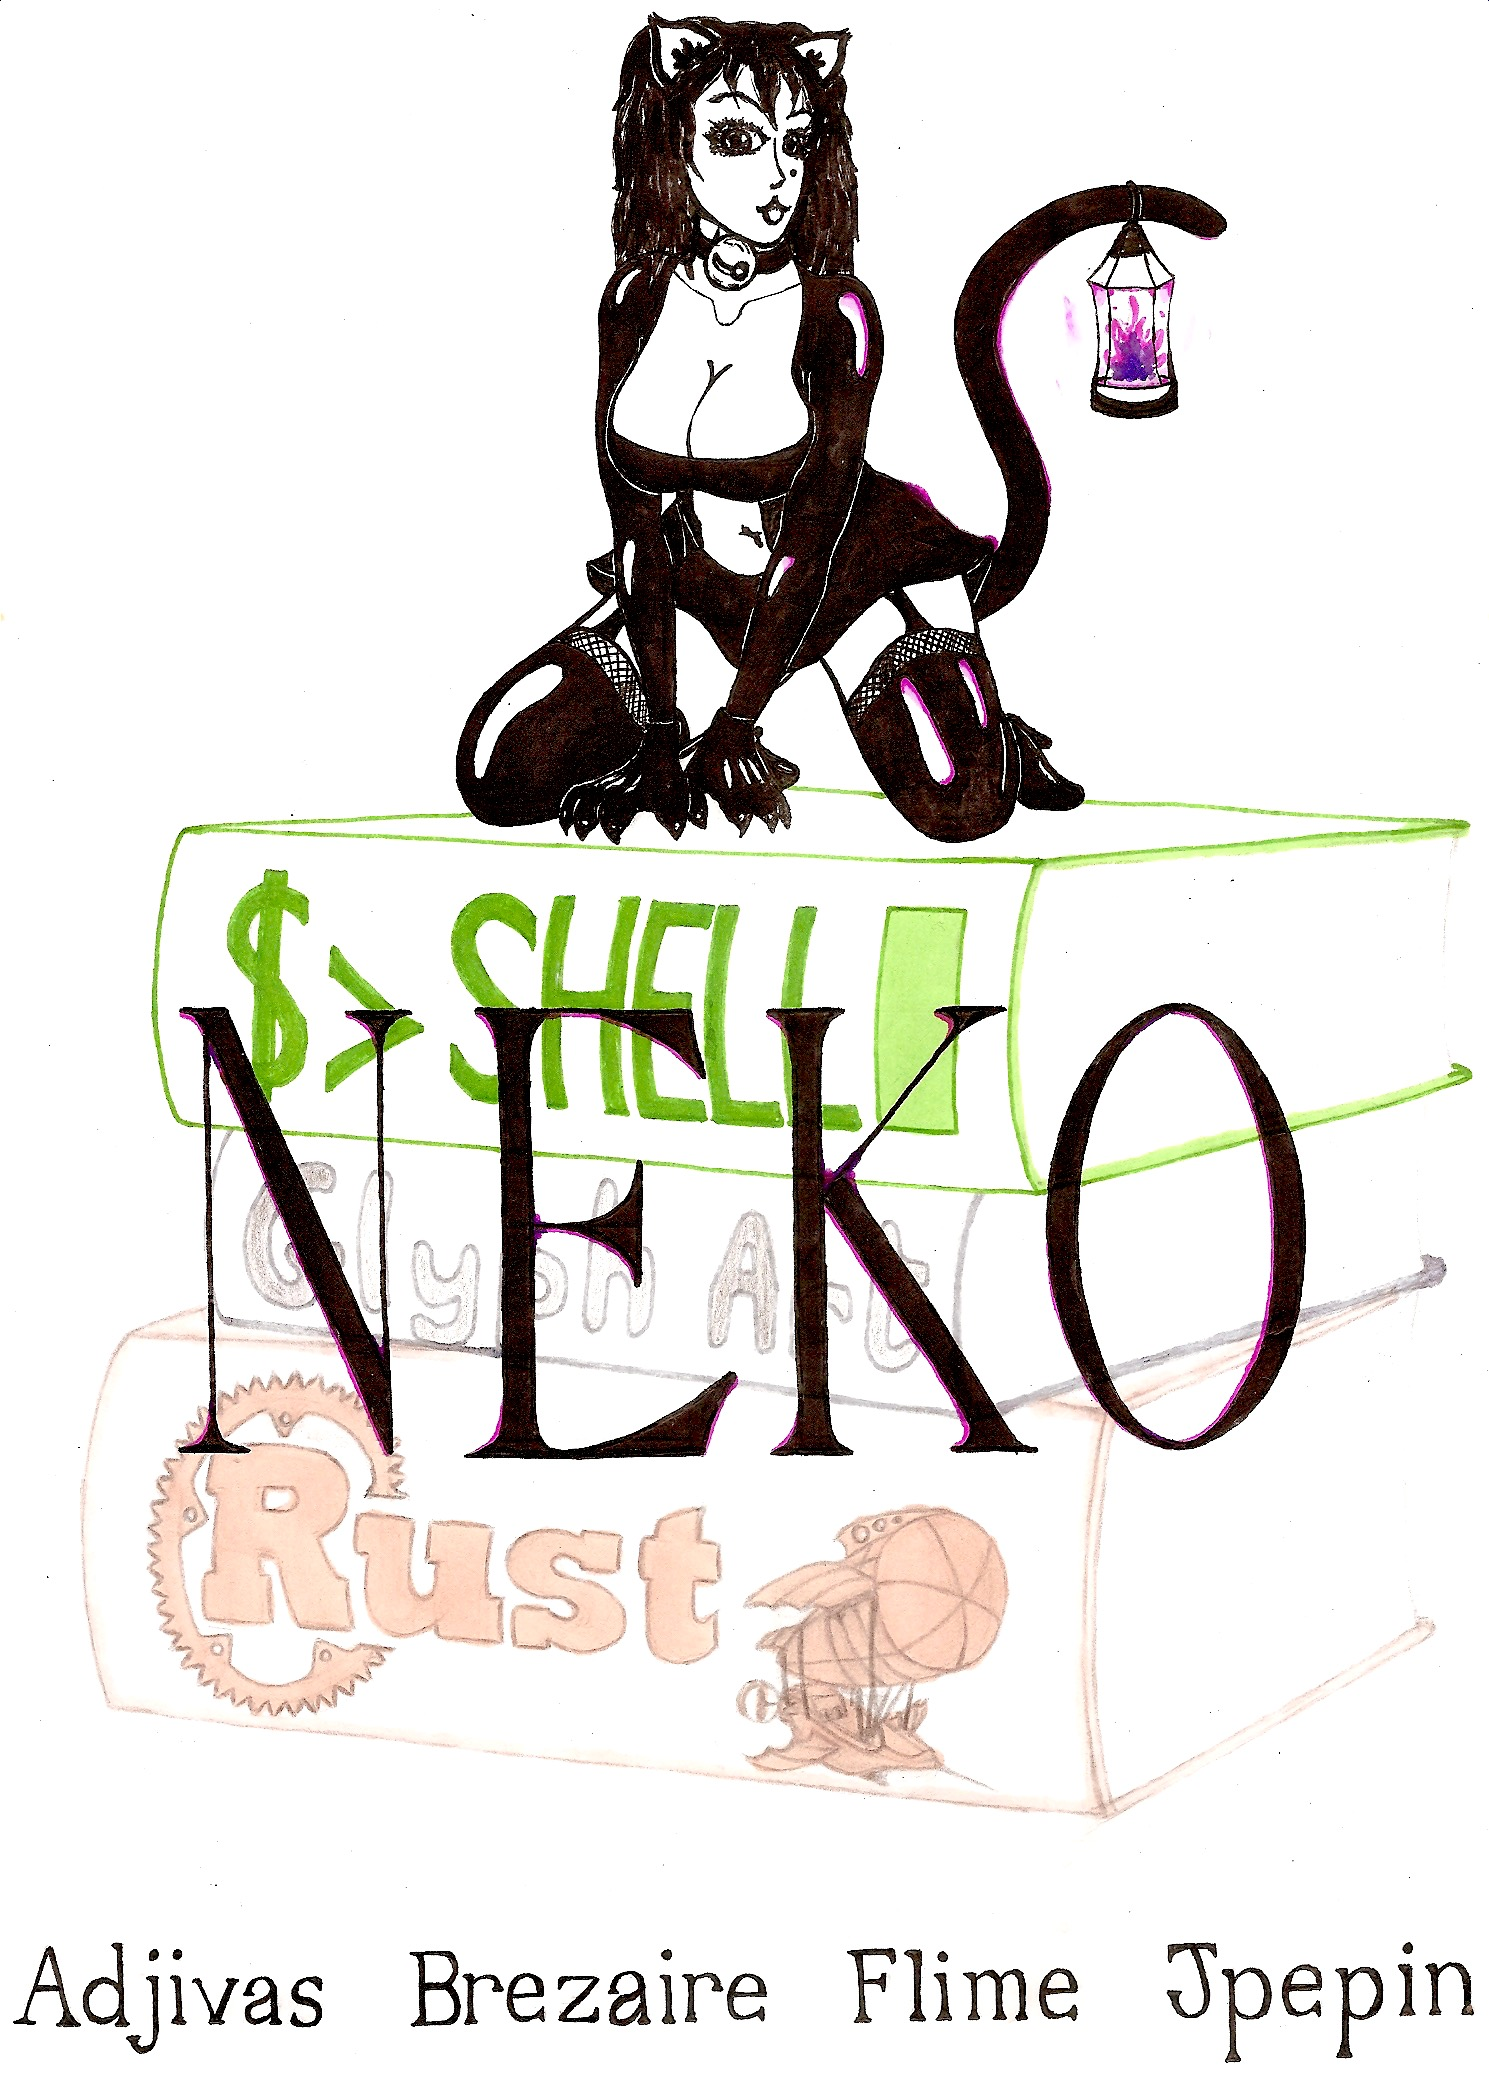
\includegraphics[scale=0.25]{images/neko.jpg}
\end{titlepage}

\tableofcontents

\titleformat{\chapter}[display]
  {\Huge}
  {\filleft\texttt{\chaptertitlename} \Huge\thechapter}
  {0ex}
  {\filleft}
  [\titlerule]

\chapter{Premiere partie}

\section{Préambule}

\begin{figure}[!ht]
  \begin{minipage}{1in}
    \centering
    \fontsize{30pt}{7pt}\selectfont
    \symbol{"E000}\symbol{"E001}\symbol{"E002}\symbol{"E003}\symbol{"E004}\symbol{"E005}\symbol{"E006}\symbol{"E007}\symbol{"E008}\symbol{"E009}\\*
    \symbol{"E00A}\symbol{"E00B}\symbol{"E00C}\symbol{"E00D}\symbol{"E00E}\symbol{"E00F}\symbol{"E010}\symbol{"E011}\symbol{"E012}\symbol{"E013}\\*
    \symbol{"E014}\symbol{"E015}\symbol{"E016}\symbol{"E017}\symbol{"E018}\symbol{"E019}\symbol{"E01A}\symbol{"E01B}\symbol{"E01C}\symbol{"E01D}\\*
    \symbol{"E01E}\symbol{"E01F}\symbol{"E020}\symbol{"E021}\symbol{"E022}\symbol{"E023}\symbol{"E024}\symbol{"E025}\symbol{"E026}\symbol{"E027}\\*
    \symbol{"E028}\symbol{"E029}\symbol{"E02A}\symbol{"E02B}\symbol{"E02C}\symbol{"E02D}\symbol{"E02E}\symbol{"E02F}\symbol{"E030}\symbol{"E031}\\*
  \end{minipage}
  \caption[Caption for LOF]{\href{https://en.wikipedia.org/wiki/Wikipedia:Wikipe-tan}{Wikipe-tan} \textendash{ウィキペたん}\textendash{}}
\end{figure}

Une nékoe \textendash{ねこみみ}\textendash{} est un persona d'animé japonais avec des traits de chat
\textendash{mimikko
	\footnote{ Kemonomimi ou mimikko est un personnage humain d'animé avec les caractéristiques d'un animal telles que sa personnalité ou encore son physique
		\textendash{獣耳}\textendash.
			}} \textendash.

Le GlyphArt est l'écriture d'une image via des caractères compris dans l'Unicode privé, ce projet démontre ce procédé via
\href{https://limaconoob.github.io/Image2font}{Image2font}. \\

L'\href{https://fr.wikipedia.org/wiki/SVG_OpenType}{SVG OpenType} est un format ouvert de police de caractères vectorielles multicolors. \\

$\name$ est une programmeuse nékoe fictive de terminal inventée pour assister des utilisateurs. \\

\section{Introduction}
\thispagestyle{empty}
$\name$ est une nékoe de terminal qui a pour but d'apporter les Arts, la Culture et une assistance à qui saura utiliser un shell.
Humanisée d’émotions et fondée sur l'expérience de la \href{https://fr.wikipedia.org/wiki/Chambre_chinoise}{chambre chinoise}, celle-ci sera donc instruite via des bibliotèques.

L'organisation GitHub $\organization$ de philosophie \href{https://fr.wikipedia.org/wiki/Libriste}{libriste} fut créée pour distribuer et maintenir communautairement les dépôts nécessaires au développement de cette Nékoe de terminal.

\begin{figure}[!ht]
    \begin{minipage}{\textwidth}
    \centering
		\begin{tabular}{p{.10\textwidth}p{.85\textwidth}}
			\textbf{\href{https://github.com/Arukana/book}{Book}} & La documentation du projet $\program$. \\
            \textbf{\href{https://github.com/Arukana/PtyProc}{PtyProc}} & L'\href{https://fr.wikipedia.org/wiki/Middleware}{intergiciel} \textendash{\href{https://en.wikipedia.org/wiki/Middleware}{Middleware}}\textendash{ } et l'\href{https://fr.wikipedia.org/wiki/Backend}{arrière-plan} \textendash{back-end}\textendash{ } de l'émulateur du terminal \href{https://fr.wikipedia.org/wiki/VT100}{VT100}. \\
            \textbf{\href{https://github.com/Arukana/Editor}{Editor}} & L'éditeur et la bibliothèque d'expression de la nékoe. \\
            \textbf{\href{https://github.com/Arukana/Neko}{Neko}} & Le programme $\program$. \\
            \textbf{\href{https://github.com/Arukana/LibNya}{LibNya}} & La bibliothèque dynamique de teste du programme $\program$. \\
            \textbf{\href{https://github.com/Arukana/ffi}{ffi}} & L'\href{https://fr.wikipedia.org/wiki/Header}{en-têtes} \textendash{ \href{https://en.wikipedia.org/wiki/Header_(computing)}{header} }\textendash{ } sont les déclarations des structures et énumérations de la nékoe. \\
	        \textbf{\href{https://github.com/Arukana/Image2font}{Image2font}} & Le convertisseur d'images en une police d’écriture. \\
            \textbf{\href{https://github.com/Arukana/nTerm}{nTerm}} & L'\href{https://fr.wikipedia.org/wiki/Interface_graphique}{interface graphique} de émulateur. \\
        \end{tabular}
		\caption*{
            Ces dépôt sont interdépendant tel que : \\
			\begin{forest}
			    [\href{https://github.com/Arukana/nTerm}{nTerm}
					[\href{https://github.com/Arukana/Neko}{Neko}
					    [\href{https://github.com/Arukana/Editor}{Editor}]
                        [\href{https://github.com/Arukana/PtyProc}{PtyProc}
						    [\href{https://github.com/hibariya/pty-rs}{Pty}]
					    ]
					]
			    ]
			\end{forest}
			\begin{forest}
                [\href{https://github.com/Arukana/LibNya}{LibNya}
                    [\href{https://github.com/Arukana/ffi}{ffi}]
                ]
			\end{forest}
		}
    \end{minipage}
\end{figure}

\subsection{Utilisation}

La constante d’environnement {\textit{\$NEKO\_PATH}} pourra être définie à \enquote{\$HOME/.neko} et comprendra les sous-répertoires {\textit{lib}}, {\textit{rep}}, {\textit{texels}} et {\textit{sprites}}. Sinon, les \href{https://fr.wikipedia.org/wiki/Biblioth%C3%A8que_logicielle}{bibliothèques} de l'organisation $\organization$ ceux reporterons à la constante \href{http://doc.crates.io/environment-variables.html}{\textit{\$CARGO\_MANIFEST\_DIR}} de valeurs relatives aux répertoires contenant les \href{https://en.wikipedia.org/wiki/Manifest_file}{fichiers manifests}.

\begin{figure}[!ht]
    \begin{minipage}{\textwidth}
    \centering
        \begin{tabular}{p{.15\textwidth}p{.85\textwidth}}
			\href{https://github.com/Arukana/Editor/tree/master/assets/sprites}{\textbf{sprite}} & Les sprites de la nékoe. \\
			\href{https://github.com/Arukana/Editor/tree/master/assets/texels}{\textbf{texels}} & Les texels de la nékoe. \\
			\textbf{lib} & Les sources des progiciels. \\
			\textbf{rep} & Les bibliothèques dynamiques des progiciels.
        \end{tabular}
    \end{minipage}
\end{figure}

\newpage
\subsubsection{Programme $\program$ \textendash{\href{https://fr.wikipedia.org/wiki/Interface_en_ligne_de_commande}{CLI}}\textendash{}}

\begin{figure}[!ht]
    \begin{minipage}{\textwidth}
    \centering
        \begin{tabular}{p{.15\textwidth}p{.20\textwidth}p{.55\textwidth}}
                \textbf{\textendash\textendash help} && Imprime ce menu d'aide \\
                \textbf{\textendash\textendash version, \textendash{V}} && Imprime la version du programme $\program$ \\
                \textbf{\textendash\textendash command, \textendash{c}} & [/bin/zsh] & Précise le processus fils. \\
                \violet
                \textbf{\textendash\textendash repeat, \textendash{r}} & [1000] & Précise le temps de répétition du maintien d'une touche enfoncée tel que $\{2\dots{}N\}$. \\
                \violet
                \textbf{\textendash\textendash interval, \textendash{i}} & [1000] & Précise le temps d'intervalle durant les répétitions tel que $\sum_{i=repeat}^{\infty} U_{interval}\times{}i$. \\
        \end{tabular}
    \end{minipage}
    \caption[Caption]{ \colorbox{violet!10}{\phantom{\_}} Fonctionnalité supplémentaire \enquote{keyboard-time}.}
\end{figure}

\subsubsection{Commande $\program$ \textendash{\href{https://en.wikipedia.org/wiki/Shell_builtin}{builtin}\textendash{}}}

Le programme $\program$ substitura la commande neko(1) pour son processus enfant uniquement et qui sera à l'occurrence notre \href{https://fr.wikipedia.org/wiki/Interpr%C3%A9teur_de_commandes}{interpréteur de commandes}.

Cette commande comprend les options si-suivantes:
\begin{figure}[!ht]
    \begin{minipage}{\textwidth}
    \centering
		\begin{tabular}{p{.30\textwidth}p{.16\textwidth}p{.44\textwidth}}
			\textbf{install <url>} & https://git... & Installe depuis dépôt git un plugiciel. \\
			\textbf{uninstall <author@libname>} & Arukana@LibNya & Désinstalle les sources et la bibliothèque dynamique d'un plugiciel \textendash{} \href{https://fr.wikipedia.org/wiki/Plugin}{plugin} \textendash{}. \\
			\textbf{mount <author@libname> [<priority>]} & Arukana@LibNya 1 & Monte une bibliothèque dynamique avec une priorité de niveau zero. \\
			\textbf{unmount <author@libname>} & Arukana@LibNya & Démonte une bibliothèque dynamique. \\
			\textbf{update <author@libname>} & Arukana@LibNya & Révise une bibliothèque dynamique. \\
		\end{tabular}
    \end{minipage}
    \caption[Caption] {
		\enquote{install} implicite \enquote{mount}. \\
		\enquote{uninstall} implicite \enquote{unmount}.
    }
\end{figure}

\newpage
\subsection{Programmeur}

Les sources d'une bibliothèque dynamique devront toujours comprendre un \enquote{Makefile} et un fichier manifest du nom de \enquote{Neko.toml}. \\

\begin{itemize}
	\item Le Makefile devra compiler une bibliothèque nommé \enquote{author@repository.dylib} via la règle \textit{default}.
	\item Une Manifest pourra configurer son niveau de priorité via la variable priority qui sera de valeur 0 par défaut.
\end{itemize}

\subsubsection{Fonctions dynamiques \textendash{\href{https://en.wikipedia.org/wiki/Foreign_function_interface}{FFI}}\textendash{}}

Le bibliothèque LibNya est pour ses branches \href{https://github.com/Arukana/LibNya/tree/c}{C} et \href{https://github.com/Arukana/LibNya}{Rust} un exemple d'utilisation de la liste des fonctions si-suivantes : \\

\begin{figure}[!ht]
    \begin{minipage}{\textwidth}
    \centering
        \begin{tabular}{p{.40\textwidth}p{.50\textwidth}}
            \textbf{void install (t\_lbstat *lib, void **data)} & Quand la bibliothèque est installée. \\
            \textbf{void uninstall (t\_lbstat *lib, void **data)} & Quand la bibliothèque va être désinstallé. \\
            \textbf{void mount (t\_lbstat *lib, void **data)} & Quand la bibliothèque est montée. \\
            \textbf{void unmount (t\_lbstat *lib, void **data)} & Quand la la bibliothèque est démontée. \\
            \textbf{void idle (t\_lbstat *lib, void **data)} & Pour chaque cycle compris entre chaques événements. \\
            \textbf{void resized (t\_lbstat *lib, void **data, Winszed *win)} & Quand la taille de la fenêtre change. \\
            \textbf{void process (t\_lbstat *lib, void **data, char *name, pid\_t pid)} & Quand le processus courrant change. \\
            \textbf{void command (t\_lbstat *lib, void **data, char *lined)} & Quand une ligne va être envoyée. \\
            \textbf{void keyUnicodeDown (t\_lbstat *lib, void **data, unsigned long long key)} & Quand une touche enfoncée va être envoyée. \\
            \textbf{void keyStringDown (t\_lbstat *lib, void **data, char *copy)} & Quand un texte va être envoyé. \\
            \violet
            \textbf{void keyRepeatDown (t\_lbstat *lib, void **data, unsigned int repeat)} & Quand une touche est maintenue enfoncée $\{2\dots{}N\}$. \\
            \violet
            \textbf{void keyIntervalDown (t\_lbstat *lib, void **data, long long repeat)} & Qurant \textit{KeyDownRepeat}, donne l'intervalle : $\sum_{i=repeat}^{\infty} U_{interval}\times{}i$. \\
            \textbf{void mousePress (t\_lbstat *lib, void **data, unsigned short cartesian[2], int code)} & Quand le curseur est pressé à une coordonnée cartésienne. \\
            \textbf{void input (t\_lbstat *lib, void **data, char *output)} & Quand un texte va être imprimé sur l'entrée standard du processus fils. \\
            \textbf{void output (t\_lbstat *lib, void **data, char *output)} & Quand un texte est imprimé depuis la sortie standard du processus fils. \\
        \end{tabular}
    \end{minipage}
   \caption[Caption]{ \colorbox{violet!10}{\phantom{\_}} Fonctionnalité supplémentaire \enquote{keyboard-time}.}
\end{figure}

\newpage
\section{$\dependency$}

L'$\dependency$ est à la fois :

\begin{enumerate}
	\item Un programme qui selon une liste de primitive permettra de devirer des expressions en commandes.
	Interface utilisateur en mode texte \textendash\href{https://en.wikipedia.org/wiki/Text-based_user_interface}{TUI}\textendash{}.
	\item Une bibliothèque et dépenpence du projet Neko, qui chargera un dictionnaire de \href{https://en.wikipedia.org/wiki/Sprite_(computer_graphics)}{sprite}.
\end{enumerate}

\subsection{Programme}
L'$\dependency$ comprend une liste de sprite, chacun de 1 à $\maxDraw$ \textendash{SPEC\_MAX\_DRAW}\textendash{} dessins ; un dessin comprenant $\maxXY$ \href{https://fr.wikipedia.org/wiki/Texel_(infographie)}{texels} \textendash{SPEC\_MAX\_XY}\textendash{}. Ainsi, par \href{https://fr.wikipedia.org/wiki/Arrangement_avec_r%C3%A9p%C3%A9tition}{arrangement avec répétition}, nous pourrons definir pour $\maxEmotion$ emotions \textendash{SPEC\_MAX\_EMOTION}\textendash{} notre nombre limite expressions à :

\begin{equation}
	\pgfkeys{/pgf/fpu=true}
	\overline{\Alpha_{\maxEmotion}^{\maxDrawMulXY}}=\maxDrawMulXY^{\maxEmotion}=\pgfmathparse{(\maxX*\maxY*\maxDraw)^\maxEmotion}\pgfmathresult
	\pgfkeys{/pgf/fpu=false}
\end{equation}

\subsubsection{Interface}

L'interface est représentée par :

\begin{itemize}
	\item Un menu de commandes.
	\item Une liste déroulante de sprite.
    \item {
		\begin{itemize}
			\item Le numéro, délais en milliseconde et posture d'un dessin.
			\item Le dessin par caractère, parti du corp et emotion.
			\item La liste des emotions disponible pour la case courrante.
		\end{itemize}
    }
    \item La somme de toute les emotions non nul par posture pour la sprite courrante. \\
\end{itemize}

Tel que :

\begin{tabbing}
    Quit <q> \\*
    bust \\*
    0 - PT0.200S: Talk \\*
    \symbol{"E000}\symbol{"E001}\symbol{"E002}\symbol{"E003}\symbol{"E004}\symbol{"E005}\symbol{"E006}\symbol{"E007}\symbol{"E008}\symbol{"E009} HeHeHe\_\_\_\_\_\_\_\_\_\_\_\_\_\_ \_\_\_\_\_\_\_\_\_\_ \\*
    \symbol{"E00A}\symbol{"E00B}\symbol{"E00C}\symbol{"E00D}\symbol{"E00E}\symbol{"E00F}\symbol{"E010}\symbol{"E011}\symbol{"E012}\symbol{"E013} HeHeHe\_\_\_\_\_\_\_\_\_\_\_\_\_\_ \_\_\_\_\_\_\_\_\_\_ \\*
    \symbol{"E014}\symbol{"E015}\symbol{"E016}\symbol{"E017}\symbol{"E018}\symbol{"E019}\symbol{"E01A}\symbol{"E01B}\symbol{"E01C}\symbol{"E01D} \_\_\_\_\_\_\_\_Mo\_\_\_\_\_\_\_\_\_\_ \_\_\_\_\_\_\_\_\_\_ \\*
    \symbol{"E01E}\symbol{"E01F}\symbol{"E020}\symbol{"E021}\symbol{"E022}\symbol{"E023}\symbol{"E024}\symbol{"E025}\symbol{"E026}\symbol{"E027} \_\_\_\_\_\_\_\_\_\_\_\_\_\_\_\_\_\_\_\_ \_\_\_\_\_\_\_\_\_\_ \\*
    \symbol{"E028}\symbol{"E029}\symbol{"E02A}\symbol{"E02B}\symbol{"E02C}\symbol{"E02D}\symbol{"E02E}\symbol{"E02F}\symbol{"E030}\symbol{"E031} \_\_\_\_\_\_\_\_\_\_\_\_\_\_\_\_\_\_\_\_ \_\_\_\_\_\_\_\_\_\_ \\*
    \\*
    S\_ \\*
    1 - PT0.200S: NotTalk \\*
    \symbol{"E000}\symbol{"E001}\symbol{"E002}\symbol{"E003}\symbol{"E004}\symbol{"E005}\symbol{"E006}\symbol{"E007}\symbol{"E008}\symbol{"E009} HeHeHe\_\_\_\_\_\_\_\_\_\_\_\_\_\_ SSS\_\_\_\_\_\_\_ \\*
    \symbol{"E00A}\symbol{"E00B}\symbol{"E00C}\symbol{"E00D}\symbol{"E00E}\symbol{"E00F}\symbol{"E010}\symbol{"E011}\symbol{"E012}\symbol{"E013} HeHeHe\_\_\_\_\_\_\_\_\_\_\_\_\_\_ SSS\_\_\_\_\_\_\_ \\*
    \symbol{"E014}\symbol{"E015}\symbol{"E016}\symbol{"E017}\symbol{"E018}\symbol{"E019}\symbol{"E01A}\symbol{"E01B}\symbol{"E01C}\symbol{"E01D} \_\_\_\_\_\_\_\_Mo\_\_\_\_\_\_\_\_\_\_ \_\_\_\_\_\_\_\_\_\_ \\*
    \symbol{"E01E}\symbol{"E01F}\symbol{"E020}\symbol{"E021}\symbol{"E022}\symbol{"E023}\symbol{"E024}\symbol{"E025}\symbol{"E026}\symbol{"E027} \_\_\_\_\_\_\_\_\_\_\_\_\_\_\_\_\_\_\_\_ \_\_\_\_\_\_\_\_\_\_ \\*
    \symbol{"E028}\symbol{"E029}\symbol{"E02A}\symbol{"E02B}\symbol{"E02C}\symbol{"E02D}\symbol{"E02E}\symbol{"E02F}\symbol{"E030}\symbol{"E031} \_\_\_\_\_\_\_\_\_\_\_\_\_\_\_\_\_\_\_\_ \_\_\_\_\_\_\_\_\_\_ \\*
    \\*
    \_S \\*
    --Talk --NotTalk Heart:Shocked
\end{tabbing}

La représentation non nul \enquote{--Talk --NotTalk Heart:Shocked} pourra être utilisé via les énumérations \textbf{Part} et \textbf{Emotion} d'écrite par la bibliothèque \href{https://github.com/Arukana/ffi}{ffi} pour reproduire la même expression depuis une bibliothèque dynamique.

\newpage

\subsubsection{Raccourcis clavier}

La saisie est adapté selon la disposition des touches du \href{https://en.wikipedia.org/wiki/ADM-3A}{terminal ADM-3A} de la société \href{https://en.wikipedia.org/wiki/Lear_Siegler}{Lear Siegler}. \\

\begin{figure}[!ht]
  \begin{minipage}{\textwidth}
    \centering
    \begin{tabular}{p{.30\textwidth}p{.65\textwidth}}
        \toprule
        \toprule
            Touche & Description \\
        \midrule
            \Ctrl+\keystroke{q}ou\keystroke{q} & Quitter le programme. \\
            \violet
            \Ctrl+\keystroke{c}ou\keystroke{c} & Copie la commande dans le presse-papier. \\
            \Home{}ou\keystroke{g} & Sélectionne la première animation. \\
            \PgUp{}ou\keystroke{H} & Sélectionne l'animation précédente. \\
            \PgDown{}ou\keystroke{L} & Sélectionne l'animation suivante. \\
            \End{}ou\keystroke{G} & Sélectionne la dernière animation. \\
            \keystroke{\{}ou\keystroke{[} & Sélectionne le sprite précédent. \\
            \keystroke{\}}ou\keystroke{]} & Sélectionne le sprite suivant. \\
            \LArrow{}ou\keystroke{h} & Sélectionne la cellule de gauche. \\
            \UArrow{}ou\keystroke{k} & Sélectionne la cellule du haut. \\
            \DArrow{}ou\keystroke{j} & Sélectionne la cellule du bas. \\
            \RArrow{}ou\keystroke{l} & Sélectionne la cellule de droite. \\
            \keystroke{0}...\keystroke{9} & Change l'émotion du groupe de cellules courrant. \\
        \bottomrule
    \end{tabular}
  \end{minipage}
  \caption[Caption]{ \colorbox{violet!10}{\phantom{\_}} Fonctionnalité supplémentaire \enquote{Clipboard}.}
\end{figure}

\newpage

\subsection{Bibliothèque}

...

\begin{figure}[!ht]
  \centering
  \begin{dot2tex}[dot,scale=0.25]
digraph graphic {
  d2tstyleonly = true;
  node [shape = "box", width = "2.5", texmode="verbatim", style = "top color=cyan!10,bottom color=cyan!35,draw=cyan!50,rounded corners"];
  graph [shape = "box", texmode="math", style = "top color=blue!10,bottom color=blue!35,draw=blue!50"];

  nodeGraphic [label="Struct Graphic<Default + Debug + Clone>\n
    texel: HashMap<Posture, HashMap<Tuple, Vec<Texel>>>,
    sprite: io::Cursor<Vec<(Sheet, Sprite)>>,

    + fn explicite_emotion(&mut self, name: &Sheet, change: &[[Tuple; SPEC_MAX_XY]; SPEC_MAX_DRAW]) -> Option<&Sprite>
  "];

  nodeTuple [label="Struct Tuple<Copy + Clone + Debug + Default + Eq + PartialEq + Hash + From>\n
    + Part,
    + Emotion,
  "];

  nodeDraw [label="Struct Draw<Default + Debug + Clone + IntoIterator>\n
    posture: Posture,
    duration: time::Duration,
    board: io::Cursor<[(Emotion, Texel); SPEC_MAX_XY]>,
  "];

  nodeTexel [label="Struct Texel<Default + Copy + Clone + Display + Debug + PartielEq>\n
    part: Part,
    glyph: char,
  "];

  nodeSprite [label="Struct Sprite<Default + Clone + IntoIterator>\n
    texel: HashMap<Tuple, Vec<Texel>>,
    sheet: io::Cursor<[Draw; SPEC_MAX_DRAW]>,
    count: usize,
  "];

  nodePart [label="Enum Part<Default + Display + Debug + Clone + Copy + Eq + PartialEq + Hash>\n
    None = b'_',
    ArmLeft = b'a',
    ArmRight = b'A',
    Boobs = b'b',
    Clavicle = b'c',
    EarLeft = b'e',
    EarRight = b'E',
    EyeLeft = b'y',
    EyeRight = b'Y',
    HairTop = b'o',
    HairLeft = b'r',
    HairRight = b'R',
    HandLeft = b'd',
    HandRight = b'D',
    Mouth = b'm',
    Tail = b't',
    Bell = b'l',
    ExclamationMark = b'x',
    ExclamationMarks = b'X',
    Heart = b'h',
    Hearts = b'H',
    Lantern = b'n',
    QuestionMark = b'q',
    QuestionMarks = b'Q',
    WoolBall = b'w',
  "];

  nodePosture [label="Enum Posture<Default + Display + Debug + Clone + Copy + Eq + PartialEq + Hash>\n
    None = b'_',
    Talk = b't',
    NotTalk = b'n',
    Bust = b'b',
    Lying = b'l',
    Seiza = b's',
    Behind = b'b',
  "];

  nodeSheet [label="Enum Sheet<Default + Display + Debug + Clone + Copy + Eq + PartialEq + Hash>\n
    None = b'_',
    Bust = b'b',
  "];

  nodeEmotion [label="Enum Emotion<Default + Display + Debug + Clone + Copy + Eq + PartialEq + Hash>\n
    None = b'_',
    Angry = b'a',
    Happy = b'h',
    Love = b'l',
    Malicious = b'm',
    Misunderstanding = b'i',
    Normal = b'n',
    Playing = b'p',
    Shocked = b'o',
    Sleepy = b's',
    Speechless = b'e',
    Surprised = b'u',
  "];

  nodePosture -> nodeGraphic;
  nodeTuple -> nodeGraphic;
  nodeTexel -> nodeGraphic;
  nodeSheet -> nodeGraphic;
  nodeSprite -> nodeGraphic;
  nodeTexel -> nodeSprite;
  nodeDraw -> nodeSprite;
  nodePart -> nodeTexel;
  nodePart -> nodeTuple;
  nodeEmotion -> nodeTuple;
  nodePosture -> nodeDraw;
  nodeTexel -> nodeDraw;
  nodeEmotion -> nodeDraw;
}
  \end{dot2tex}
  \caption[Caption for LOF]{

  }
  \label{graphic}
  \caption[Caption for LOF]{ Diagramme UML \footnotemark{} simplifié du module graphique. }
\end{figure}

\footnotetext{En génie logiciel, le langage de modélisation orienté objet unifié de l'anglais
	\enquote{Unified Modeling Language}
		\textendash{ UML }\textendash{ } est la représentation schématique d'un programme par de l'orienté objet}

\end{document}
